\documentclass[11pt]{article}
\usepackage{graphicx}
\usepackage[a4paper, margin=1in]{geometry}
\usepackage{fontspec} % Times-style font (TeX Gyre Termes, a Times clone), replaces the template's 'times' package
\setmainfont{texgyretermes}[Extension=.otf, UprightFont=*-regular, BoldFont=*-bold, ItalicFont=*-italic, BoldItalicFont=*-bolditalic]
\usepackage{authblk} % Package for superscript affiliations

\begin{document}

% Header with logo
\begin{minipage}{0.2\textwidth}
    
\includegraphics[width=\textwidth]{ercoftac_logo.png}
\end{minipage}
\hfill
\begin{minipage}{0.75\textwidth}
    \fontsize{8}{10}\selectfont
    \textbf{4th ERCOFTAC Workshop on Machine Learning for Fluid Dynamics, April 2027, Florence, Italy}
\end{minipage}

\begin{center}
  { \fontsize{14}{16} \textbf{What Limits a Fourier Neural Operator for Parametric Darcy Flow?\\ Training Recipe, Data, Label Noise and a Calibrated Solver Comparison} } \\
    \vspace{0.3cm}
    \normalsize \textbf{Aryamann Srivastava$^{1}$, Varun Sathaye$^{1}$, Atishay Jain$^{1}$, Vedant S.\ Tiwari$^{1}$} \\
  { \fontsize{9}{10}\selectfont  \textit{$^1$ Department of Aerospace Engineering, IIT Kanpur, India} } \\
\end{center}

\vspace{-2mm}
\noindent\fontsize{10.5}{12.6}\selectfont
We study how well a Fourier Neural Operator (FNO) \cite{li2021fno} can learn the permeability-to-pressure map of steady Darcy flow, $-\nabla\!\cdot(\kappa\nabla u)=1$, on real PDEBench data \cite{takamoto2022pdebench} ($\kappa\in\{0.1,1\}$, $64\times64$, 900/100/200 train/validation/test maps), and what actually limits its accuracy. An MLP is the baseline.
\textbf{Training, not architecture, dominated.} Our first FNO reached a relative $L_2$ error of 0.052. Matching the loss to the metric (relative $L_2$), using a single cosine learning-rate decay instead of repeated restarts, and augmenting with the exact D4 symmetries of the problem halved the error at equal budget (FNO $0.052\to0.025$, MLP $0.080\to0.045$; Fig.~1a). Fourier modes (4--32), width ($\ge32$), learning rate and batch size changed the error by less than 0.004, while depth and training length gave slow gains. The final FNO (9.5\,M parameters) reaches $0.0202\pm0.0004$ against $0.0415\pm0.0009$ for a tuned 100.7\,M-parameter MLP (5 seeds). An FNO trained on 400 maps (0.026) beats an MLP trained on 9\,700 (0.036); the FNO plateaus near 0.02 beyond 5\,000 maps, but is 2--3 times worse on a grid it was not trained on.
\textbf{Solver comparison.} Against a finite-volume solver calibrated to the dataset, the FNO is closer to the reference at the same resolution (0.020 vs.\ 0.044 at $64^2$) and 5--35 times faster on a GPU, but not faster on a single CPU core (37 vs.\ 7\,ms); an earlier speed-up claim based on an inefficient reference solver was withdrawn. Predictions keep the boundary level (0.1157 vs.\ 0.1159), positivity ($1.5\times10^{-5}$ negative pixels) and the mean pressure (1.7\,\%). The error is concentrated in the 4\,\% of test maps that are almost entirely low-permeability (0.17 vs.\ 0.019 for the rest).
\textbf{Robustness.} With Gaussian noise of up to 10\,\% on the training pressure labels the FNO error rises only from 0.025 to 0.036 (MLP: 0.045 to 0.051), staying ahead at every noise level and averaging the noise out (Fig.~1b). Self-adjusting per-sample loss weights found the hard maps by themselves (weight $2.7\times$) but did not reduce their error (0.170 vs.\ 0.172) and slightly raised the overall error; we report this as a negative result. \textbf{Limits.} One PDE and dataset, agreement with the generating solver rather than the exact PDE, and a fixed training grid.

\begin{figure}[htbp]
    \centering
    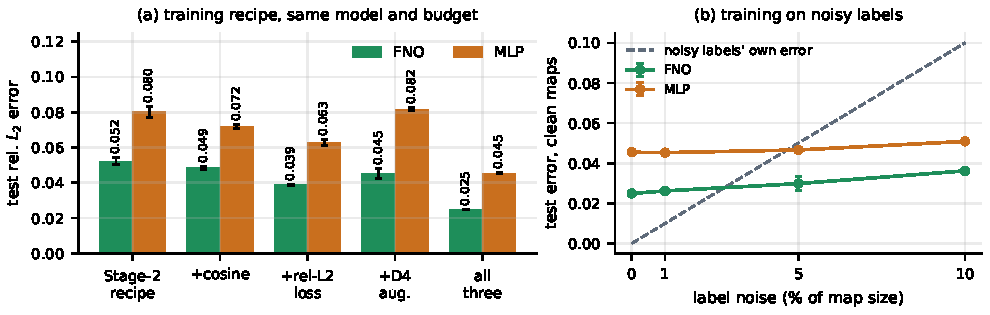
\includegraphics[width=0.98\textwidth]{fig_abstract.pdf}
    \caption{(a) Training recipe, same model and budget (3 seeds). (b) Test error on clean maps after training on noisy labels.}
    \label{fig:abs}
\end{figure}
\vspace{-8mm}
\bibliographystyle{unsrt}
\bibliography{references.bib}

\end{document}
